\chapter{Introduction}
%\paragraph{Scheduling on a high level}
Computer programs need computing, storage and communication resources to function. 
Usually the availability of such resources is limited and the system has to share these resources among multiple users. 
Resource management is an important aspect of a system.
Scheduling falls under the umbrella of resource management. 
It can be viewed as a governance model that \textit{governs} how the resources are shared among users and how various parts of the system function together. 
The governance model is designed so as to meet goals about resource management and performance of the system. 
As an example, an operating system uses resources such as memory, CPUs, and disk.
It allows multiple processes to use these resources at the same time through sophisticated scheduling techniques. 

%\paragraph{Scheduling's history}
Scheduling has been studied extensively in many communities including computer science theory, computer systems, and industrial engineering. 
Typically a scheduling problems involves finding a schedule with a certain objective.
The desired solution is the one that either meets the objective or gets close to it.
Many scheduling problems are difficult in nature.
For example, the problem of scheduling $N$ jobs each with a unit execution time on $k$ processors such that the makespan of the schedule is minimized is NP complete~\cite{ULLMAN1975384}.
Some of the standard techniques used to solve scheduling problems are: using domain specific heuristics, dynamic programming, greedy algorithms, and approximation algorithms. 

%\paragraph{Scheduling for databases}
In this dissertation, we establish the role of scheduling for modern database systems.
We show that scheduling can play a critical role in the functioning of the database system and can be used to meet various objectives such as resource allocation and query performance.

Before understanding the scheduling problem itself, we dive into the \textit{modern} aspect of modern database systems.

\section{Modern Database Systems and the need for Scheduling}
We distinguish traditional database systems and modern database systems based on three aspects which are closely related to the scheduling problem: modern hardware, growing data volumes, and deployment environments.
We discuss these aspects below and explain how they are related to the scheduling problem. 
\paragraph{Modern hardware:} 
Over the past few years hardware has drastically evolved. 
Modern hardware includes large main memories, Non-Uniform Memory Access (NUMA) patterns and large number of CPU cores.
%To leverage the capabilities of the modern hardware comprehensively, database architecture needs a fundamental shift from its traditional roots. 
Traditional database architecture comes from a time when memories were smaller, data were mostly resident on disks and multi-core parallelism was uncommon. 
Therefore modern systems have high availability of two resources: CPU parallelism and memory.
Scheduling involves managing resources, therefore we believe that there is a place for schedulers in modern database architecture. 
\paragraph{Growing data volumes:}
We are in the era of big data and witnessing tremendous amount of data generation.
To process the large amount of data efficiently, data processing engines must effectively leverage all the hardware features. 
However, what we are experiencing is a growing \textit{deficit} between the pace of hardware performance improvements and the pace that is demanded of data processing kernels to keep up with the growth in data volumes.

\begin{figure}
	\centering
	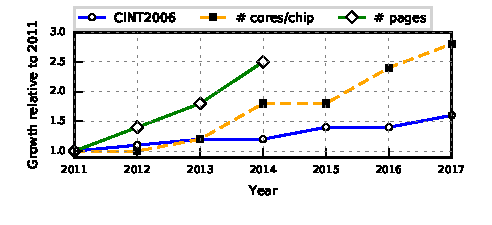
\includegraphics[width=0.75\textwidth]{system/figures/deficit.pdf}
	\caption{\textbf{Deficit - Widening gap between hardware evolution and data generation}}
	\label{fig-deficit}
\end{figure}

Figure~\ref{fig-deficit} illustrates this deficit issue by comparing improvements in processor performance (blue line) with the growth rate of data (green line), using the number of pages indexed by Google as an illustrative example. 
The processor performance improvements presented in Figure~\ref{fig-deficit} are measured by the highest reported CINT2006 benchmark result for Intel Xeon chips from~\cite{cpu2006}.
We use the number of pages indexed by Google (using estimates made by~\cite{google-pages-db}) as a proxy for data growth. 
Figure~\ref{fig-deficit} does not show the increase in the number of queries (which is about 2.5X for Google search queries from 2011--14), and the increase in the complexity of queries as applications request richer analytics. These aspects make the deficit problem worse. The figure also shows the maximum number of cores per chip used in reported CINT2006 results over time. Interestingly (and not shown in the figure), both the minimum and the average amount of memory per chip in the reported CINT2006 results has grown by $\approx$4X from 2011 to 2017.

The presented data growth rate is conservative for many organizations, which tend to see a far higher rate of increase in the data volume; for example, Facebook's warehouse grew by 3X in 2014~\cite{fb-growth-14}. 
Figure~\ref{fig-deficit} also shows (using a dotted orange line with squares) the growth in the number of cores per processor over time. 
As one can observe, the number of cores per processor is rising rapidly.
In addition, since 2011 the main memory sizes are also growing rapidly, and there is an increasing shift to larger main memory configurations. 

In addition to the data growth, there is a growing interest in finding more insights from the data as quickly as possible.
In addition to the traditional online analytical processing (OLAP), there is an increased interest in advanced analytics~\cite{DBLP:conf/sigmod/Kumar0017} (which involves machine learning algorithms), both from academic community as well as industry. 
Thus, there is a critical need for in-memory data processing methods that \textit{scale-up} to exploit the full (parallel) processing power that is locked in commodity multi-core servers today.

\paragraph{Deployment environments:} 
The most common deployment method few years ago was "on-premise database", in which an enterprise would host and maintain the database software on private servers. 
Deployment concerns such as failover handling, installing additional capacity, upgrading hardware would be taken care by the in-house database administrator. 

Today cloud databases have drastically changed the \textit{modus operandi} of database deployment.
Cloud providers host and manage databases on cloud platforms and abstract away all the deployment pain points from the users.
The database engine may be hosted on a number of hardware platforms or virtualized environments in the cloud.

Cloud databases promise the quality of their service in the form of a Service Layer Aggrement (SLA).
The most common form of SLA today is in terms of availability, which quantifies the extent to which the cloud database service would be available in a given time window. 
As the extent of availability increases, the cost to the customer increases.
We now discuss the implications of such a SLA in terms of resource management.
To meet the SLA, the database service may need to elastically add more nodes. 
Occasionally to reduce operational expenses and to lower the energy consumption, the database service may need to downsize the number of operational nodes.
Some cloud databases provide differentiated service guarantees to users based on the Service Layer Agreement (SLA). 
To guarantee the SLA for all users, the database service may require to reshuffle resources from one customer to another. 

Considering the above challenges, the resource management layer of the cloud database needs to be flexible enough to withstand dynamicity in the resource availability.
Hence the scheduler should have built in resource allocation flexibility, helping the resource management of the database become dynamic.

Next we take a deeper look into the scheduling problem in database systems.
The scope of our work is relational analytics (warehouse settings) where data primarily resides in memory. 
In relational analytics, questions on data are posed via \textit{queries}, that are made up of relational operators. 
To get an idea of the problem of scheduling in database systems, we compare traditional database systems with MapReduce~\cite{mapreduce} based systems such as Hive~\cite{thusoo2010hive}\footnote{We acknowledge that Hive now supports Tez and Spark run time environments in addition to MapReduce.} in the next section.

\section{Scheduling: Databases and MapReduce}
We focus on two aspects of scheduling to compare databases and MapReduce frameworks: a) an abstraction for tasks b) connecting resource management with relational operators' semantics.

MapReduce is a parallel data processing framework where a job is broken up in several parallel map and reduce tasks. 
MapReduce programs consists of only map tasks and reduce tasks.
The mappers and reducer tasks form the scheduling abstractions for the MapReduce framework.

In databases, a query is made up of several relational operators such as selection, join, aggregation. 
Each logical operator may have multiple physical implementations. 
For example an equi-join operator can be performed using hash-join and sort-merge join.
Given the variety in terms of relational operators and their physical implementations, databases so far did not have a common scheduling abstraction for tasks within a query. 
We hypothesize that the lack of a common scheduling abstraction is a reason why scheduler is not considered a first class citizen in database architecture.

By having a scheduling abstraction the database system can have a greater control over how resources are managed, and allotted to its users.
The abstraction makes it easy to estimate resource availability.
If the scheduling abstraction is amenable to parallelism, it may help the system to leverage parallelism offered by the hardware. 

Next we discuss specialized resource management for relational operators. 
Database community has for long focused on finding specialized resource management techniques to improve performance of either individual relational operators or query as a whole~\cite{davison1995dynamic, Bouganim:1998:MSL:288627.288646, memory-hash-ibm, mehta1993dynamic, DBLP:conf/cikm/NagD98}.
Such a specialization is difficult to achieve in MapReduce framework, in which every task is either a mapper or a reducer.
It is difficult to reason about what is the logical task being performed through the mappers and reducers. 
For example a mapper could belong to the probe phase of a join or aggregation operator. 

Through our work, we would like to achieve the best of both (databases and MapReduce framework) worlds.
We want scheduler as a first class primitive in the database architecture and the ability to perform operator centric resource management in query execution. 

We now present the contributions of this dissertation. 

\paragraph{Design and Implementation of the Quickstep Database System:}
The work in this thesis is carried out in the Quickstep Database System~\cite{quickstep-vldb, patel1quickstep, Quickstep-website}.
We begin by presenting the design and implementation of Quickstep.

Quickstep targets high performance for in-memory relational analytics. 
We describe the various components of the system including storage manager, query optimizer, query execution engine (which consists the query scheduler), and the expression evaluation module. 
Through benchmarking against other systems, we show that Quickstep is faster than other systems, often by an order of magnitude.

\paragraph{Design and Implementation of the Quickstep Scheduler:}
The core focus of this dissertation is Quickstep's query scheduler. 
We describe the \textit{nuts and bolts} of the scheduler.
We propose a novel task abstraction called \textit{work orders} used for query processing in Quickstep.
The work done in a query is broken up in several work orders.
Thus the work orders abstraction is used by all the relational operators implemented in Quickstep and it enables the system to exploit the large degree of parallelism offered by modern hardware.

\paragraph{Using the Quickstep Scheduler to meet different objectives:}
We showcase the versatility of the Quickstep scheduler by demonstrating how it can be used to meet various objectives.
Specifically we show the Quickstep scheduler in two scenarios.
First, we show how the scheduler can allocate resources such as CPU to concurrent queries through well defined policies such as fair and prioirity-based policies.
We propose a probabilistic scheduling approach, which gives the resource administrators a knob to allocate resources to concurrently running queries in the system.
We believe that this work can be useful in the age of cloud databases, where the \textit{pay as you go} philosophy for resource consumption can become the norm.

Second, we analyze the impact of scheduling strategies on query performance.
For this analysis we focus on \textit{pipelining}, a well known technique in database systems that deals with the interaction of two adjacent relational operators in a query plan DAG. 
Disk-based database systems prefer pipelined query processing over non-pipelining query processing.
We question this preference in the in-memory based systems and show that the gap between pipelining and non-pipelining is not as wide.
We study the connection between pipelining performance and parameters such as degree of parallelism, storage formats, block size and hardware prefetching.
We propose an algorithm that given a query plan and the resource availability, produces a sequence of pipelines that can provide good query performance.

Readers are advised that the content in this dissertation is based on previously published papers~\cite{quickstep-vldb, original, supplement} and another manuscript under submission.
Large sections of this dissertation are taken directly from these papers. 
Quickstep is an open source project with its source code available at \url{https://github.com/apache/incubator-quickstep}.
